\documentclass{beamer}
\usepackage[utf8]{inputenc}

\usetheme{Madrid}
\usecolortheme{default}
\usepackage{amsmath,amssymb,amsfonts,amsthm}
\usepackage{txfonts}
\usepackage{tkz-euclide}
\usepackage{listings}
\usepackage{adjustbox}
\usepackage{array}
\usepackage{tabularx}
\usepackage{gvv}
\usepackage{lmodern}
\usepackage{circuitikz}
\usepackage{tikz}
\usepackage{graphicx}
\usepackage{multicol}

\setbeamertemplate{page number in head/foot}[totalframenumber]

\usepackage{tcolorbox}
\tcbuselibrary{minted,breakable,xparse,skins}



\definecolor{bg}{gray}{0.95}
\DeclareTCBListing{mintedbox}{O{}m!O{}}{%
  breakable=true,
  listing engine=minted,
  listing only,
  minted language=#2,
  minted style=default,
  minted options={%
    linenos,
    gobble=0,
    breaklines=true,
    breakafter=,,
    fontsize=\small,
    numbersep=8pt,
    #1},
  boxsep=0pt,
  left skip=0pt,
  right skip=0pt,
  left=25pt,
  right=0pt,
  top=3pt,
  bottom=3pt,
  arc=5pt,
  leftrule=0pt,
  rightrule=0pt,
  bottomrule=2pt,
  toprule=2pt,
  colback=bg,
  colframe=orange!70,
  enhanced,
  overlay={%
    \begin{tcbclipinterior}
    \fill[orange!20!white] (frame.south west) rectangle ([xshift=20pt]frame.north west);
    \end{tcbclipinterior}},
  #3,
}
\lstset{
    language=C,
    basicstyle=\ttfamily\small,
    keywordstyle=\color{blue},
    stringstyle=\color{orange},
    commentstyle=\color{green!60!black},
    numbers=left,
    numberstyle=\tiny\color{gray},
    breaklines=true,
    showstringspaces=false,
}
%------------------------------------------------------------
%This block of code defines the information to appear in the
%Title page
\title %optional
{2.10.59}
\date{October 10,2025}


\author 
{Josyula G S Avaneesh - EE25BTECH11030}



\begin{document}



\frame{\titlepage}
\begin{frame}{Question}
Two adjacent sides of a parallelogram ABCD are given by $\vec{B-A}=\myvec{2\\10\\11}$ and $\vec{D-A}=\myvec{-1\\2\\2}$. The side $\vec{D-A}$ is rotated by an acute angle $\alpha$ in the plane of the parallelogram so that $\vec{D-A}$ becomes $(\vec{D-A})^|$. If $(\vec{D-A})^|$ makes a right angle with the side $\vec{B-A}$ then the cosine of the angle $\alpha$ is given by\\
\begin{enumerate}
\begin{multicols}{2}
    \item $\frac{8}{9}$
    \item $\frac{\sqrt{17}}{9}$
    \item $\frac{1}{9}$
    \item $\frac{4 \sqrt{5}}{9}$
\end{multicols}
\end{enumerate}
\end{frame}



\begin{frame}{Equation}
\textbf{Property:} The cosine of the angle between vector 1 and vector 2 is given by $\dfrac{{n_1}^\top n_2}{\norm{n_1}\norm{n_2}} $.
\end{frame}
\begin{frame}{Theoretical Solution}

Given details:
ABCD is a parallelogram.
\begin{align}
   \vec{B-A}=\myvec{2\\10\\11}\\
   \vec{D-A}=\myvec{-1\\2\\2}
\end{align}
The side $\vec{(D-A)}^|$ is perpendicular to $\vec{B-A}$.\\
\textbf{Property:} The cosine of the angle between vector 1 and vector 2 is given by $\dfrac{{n_1}^\top n_2}{\norm{n_1}\norm{n_2}} $.\\
Since $(\vec{D-A})^|$ is perpendicular to $\vec{B-A}$,\\


Let the angle between the vectors be $\theta$.
$$\alpha+\theta=\frac{\pi}{2}$$
\begin{align}
  \cos\theta=\frac{\vec{B-A}^\top\vec{D-A}}{\norm{B-A}\norm {D-A}}\\
  \cos\theta=\frac{\myvec{2&10&11}\myvec{-1\\2\\2}}{\sqrt{225}\sqrt{9}}\\
\end{align}
\end{frame}

\begin{frame}{Theoretical Solution} 
Let the angle between the vectors be $\theta$.
$$\alpha+\theta=\frac{\pi}{2}$$
\begin{align}
  \cos\theta=\frac{\vec{B-A}^\top\vec{D-A}}{\norm{B-A}\norm {D-A}}\\
  \cos\theta=\frac{\myvec{2&10&11}\myvec{-1\\2\\2}}{\sqrt{225}\sqrt{9}}\\
\end{align}
\end{frame}


\begin{frame}{Theoretical Solution} 
\begin{align}
   \cos\theta=\frac{40}{45}=\frac{8}{9}\brak{\because\sin\theta=\sqrt{1-\cos^2\theta}}\\
  \sin\theta=\sqrt{1-\frac{64}{81}}\\
  \sin\theta=\frac{\sqrt{17}}{9}
\end{align}
Since $\cos\alpha=\sin\theta=\frac{\sqrt{17}}{9}$\\
Ans. option 2
\end{frame}


\begin{frame}[fragile]
    \frametitle{C Code (1) - Function to store the points }

    \begin{lstlisting}

#include <math.h>

// Define a structure for a 3D vector to pass data
// between Python and C.
typedef struct {
    double x, y, z;
} Vector;

// Helper function to calculate the cross product of two vectors.
Vector cross_product(Vector a, Vector b) {
    Vector result;
    result.x = a.y * b.z - a.z * b.y;
    result.y = a.z * b.x - a.x * b.z;
    result.z = a.x * b.y - a.y * b.x;
    return result;
}




    \end{lstlisting}
\end{frame}

\begin{frame}[fragile]
    \frametitle{C Code (1) - Function to store the points }

    \begin{lstlisting}
// Helper function to calculate the magnitude (length) of a vector.
double magnitude(Vector a) {
    return sqrt(a.x * a.x + a.y * a.y + a.z * a.z);
}

Vector normalize(Vector a) {
    double mag = magnitude(a);
    Vector result = {0, 0, 0};
    // Avoid division by zero for safety
    if (mag > 1e-9) { 
        result.x = a.x / mag;
        result.y = a.y / mag;
        result.z = a.z / mag;
    }
    return result;
}



    \end{lstlisting}
\end{frame}

\begin{frame}[fragile]
    \frametitle{C Code (1) - Function to store the points }

    \begin{lstlisting}
__attribute__((visibility("default")))
Vector calculate_ad_prime(Vector ab, Vector ad) {
    // 1. Find the normal to the parallelogram's plane (AB x AD).
    Vector normal_vec = cross_product(ab, ad);

    // 2. Find a vector in the plane that is perpendicular to AB.
    // This is achieved by the cross product of the normal and AB.
    Vector ad_perp_direction = cross_product(normal_vec, ab);

    // 3. Normalize this perpendicular vector to get a pure direction.
    Vector ad_prime_unit = normalize(ad_perp_direction);

    // 4. The final AD' must have the same length as the original AD.
    double ad_mag = magnitude(ad);

 
    \end{lstlisting}
\end{frame}

\begin{frame}[fragile]
    \frametitle{C Code (1) - Function to store the points }

    \begin{lstlisting}
   // 5. Scale the unit direction vector by the correct magnitude.
    Vector ad_prime;
    ad_prime.x = ad_prime_unit.x * ad_mag;
    ad_prime.y = ad_prime_unit.y * ad_mag;
    ad_prime.z = ad_prime_unit.z * ad_mag;
    
    return ad_prime;
}




    \end{lstlisting}
\end{frame}


\begin{frame}[fragile]
    \frametitle{Python Code - Using Shared Object}
    \begin{lstlisting}

import ctypes
import numpy as np
import matplotlib.pyplot as plt
from mpl_toolkits.mplot3d.art3d import Poly3DCollection
import os # Import os to check for directory

# --- Ctypes setup to interface with the C library ---

# Define the Vector structure in Python, ensuring it mirrors the C struct
class Vector(ctypes.Structure):
    _fields_ = [("x", ctypes.c_double),
                ("y", ctypes.c_double),
                ("z", ctypes.c_double)]


\end{lstlisting}
\end{frame}

\begin{frame}[fragile]
    \frametitle{Python Code - Using Shared Object}
    \begin{lstlisting}
# --- Helper function to draw angle arcs in 3D ---
def draw_angle_arc(ax, center, v1, v2, radius, color, label, label_pos_factor=1.3):
    """Draws an arc between two vectors in 3D space."""
    v1_u = v1 / np.linalg.norm(v1)
    v2_u = v2 / np.linalg.norm(v2)
    
    angle = np.arccos(np.clip(np.dot(v1_u, v2_u), -1.0, 1.0))
    
    axis = np.cross(v1_u, v2_u)
    if np.linalg.norm(axis) < 1e-6: return
    axis_u = axis / np.linalg.norm(axis)
    
    t = np.linspace(0, angle, 50)
    arc_points = np.array([
        center + radius * (np.cos(ti) * v1_u + np.sin(ti) * np.cross(axis_u, v1_u) + (1 - np.cos(ti)) * np.dot(axis_u, v1_u) * axis_u)
        for ti in t])
\end{lstlisting}
\end{frame}
\begin{frame}[fragile]
    \frametitle{Python Code - Using Shared Object}
    \begin{lstlisting}


ax.plot(arc_points[:, 0], arc_points[:, 1], arc_points[:, 2], color=color, linewidth=2)
    
    mid_angle = angle / 2
    label_vec = (np.cos(mid_angle) * v1_u + np.sin(mid_angle) * np.cross(axis_u, v1_u) + (1 - np.cos(mid_angle)) * np.dot(axis_u, v1_u) * axis_u)
    label_pos = center + label_pos_factor * radius * label_vec
    ax.text(label_pos[0], label_pos[1], label_pos[2], label, color=color, fontsize=16, ha='center', va='center')







\end{lstlisting}
\end{frame}

\begin{frame}[fragile]
     \frametitle{Python Code - Using Shared Object}
     \begin{lstlisting}
# --- Main Logic ---
# Define the vectors from the problem
O = np.array([0, 0, 0])
AB = np.array([2, 10, 11])
AD = np.array([-1, 2, 2])

# Use the C library to calculate AD'
ab_c = Vector(*AB)
ad_c = Vector(*AD)
ad_prime_c = vector_lib.calculate_ad_prime(ab_c, ad_c)
AD_prime = np.array([ad_prime_c.x, ad_prime_c.y, ad_prime_c.z])

# Calculate the fourth vertex of the parallelogram
C = AB + AD



     \end{lstlisting}
     \end{frame}

\begin{frame}[fragile]
     \frametitle{Python Code - Using Shared Object}
     \begin{lstlisting}
   # --- Plotting ---

fig = plt.figure(figsize=(13, 11))
ax = fig.add_subplot(111, projection='3d')
fig.patch.set_facecolor('white')
ax.set_facecolor('#f0f0f0')

ax.quiver(O[0], O[1], O[2], AB[0], AB[1], AB[2], color='r', arrow_length_ratio=0.08, label='AB', linewidth=2)
ax.quiver(O[0], O[1], O[2], AD[0], AD[1], AD[2], color='b', arrow_length_ratio=0.15, label='AD', linewidth=2)
ax.quiver(O[0], O[1], O[2], AD_prime[0], AD_prime[1], AD_prime[2], color='g', linestyle='--', arrow_length_ratio=0.15, label="AD' (rotated)", linewidth=2)

verts = [O, AB, C, AD]
ax.add_collection3d(Poly3DCollection([verts], facecolors='cyan', linewidths=1.5, edgecolors='k', alpha=.25))

draw_angle_arc(ax, O, AD, AB, 3.0, 'purple', 'θ')
draw_angle_arc(ax, O, AD, AD_prime, 2.5, 'orange', 'α')


     \end{lstlisting}
     \end{frame}

\begin{frame}[fragile]
     \frametitle{Python Code - Using Shared Object}
     \begin{lstlisting}
# --- Plotting ---

fig = plt.figure(figsize=(13, 11))
ax = fig.add_subplot(111, projection='3d')
fig.patch.set_facecolor('white')
ax.set_facecolor('#f0f0f0')

ax.quiver(O[0], O[1], O[2], AB[0], AB[1], AB[2], color='r', arrow_length_ratio=0.08, label='AB', linewidth=2)
ax.quiver(O[0], O[1], O[2], AD[0], AD[1], AD[2], color='b', arrow_length_ratio=0.15, label='AD', linewidth=2)
ax.quiver(O[0], O[1], O[2], AD_prime[0], AD_prime[1], AD_prime[2], color='g', linestyle='--', arrow_length_ratio=0.15, label="AD' (rotated)", linewidth=2)

verts = [O, AB, C, AD]
ax.add_collection3d(Poly3DCollection([verts], facecolors='cyan', linewidths=1.5, edgecolors='k', alpha=.25))



     \end{lstlisting}
     \end{frame}


\begin{frame}[fragile]
     \frametitle{Python Code - Using Shared Object}
     \begin{lstlisting}
draw_angle_arc(ax, O, AD, AB, 3.0, 'purple', 'θ')
draw_angle_arc(ax, O, AD, AD_prime, 2.5, 'orange', 'α')

v_ab_u = AB / np.linalg.norm(AB)
v_ad_prime_u = AD_prime / np.linalg.norm(AD_prime)
p1 = 2.0 * v_ab_u
p2 = 2.0 * (v_ab_u + v_ad_prime_u)
p3 = 2.0 * v_ad_prime_u
ax.plot([p1[0], p2[0], p3[0]], [p1[1], p2[1], p3[1]], [p1[2], p2[2], p3[2]], color='g', linewidth=2)

ax.set_xlabel('X axis', fontsize=12, fontweight='bold')
ax.set_ylabel('Y axis', fontsize=12, fontweight='bold')
ax.set_zlabel('Z axis', fontsize=12, fontweight='bold')
ax.legend(fontsize=11)



     \end{lstlisting}
     \end{frame}

     \begin{frame}[fragile]
     \frametitle{Python Code - Using Shared Object}
     \begin{lstlisting}
max_limit = max(np.linalg.norm(AB), np.linalg.norm(C)) * 1.1
ax.set_xlim([-max_limit, max_limit])
ax.set_ylim([-max_limit, max_limit])
ax.set_zlim([-max_limit, max_limit])

ax.view_init(elev=1, azim=86)
plt.tight_layout()

# Create 'figs' directory if it doesn't exist
if not os.path.exists('figs'):
    os.makedirs('figs')
# CORRECTED typo from .savefigs to .savefig
plt.savefig('figs/plot.png')

plt.show()

     \end{lstlisting}
     \end{frame}


\begin{frame}{Plot-Using Both C and Python}
    \centering
    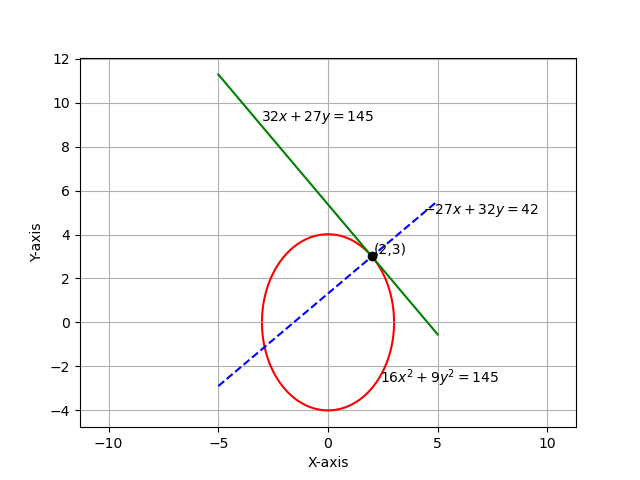
\includegraphics[width=\columnwidth, height=0.8\textheight, keepaspectratio]{figs/plot.png}     
\end{frame}

\begin{frame}[fragile]
    \frametitle{Python Code}
    \begin{lstlisting}
import numpy as np
import matplotlib.pyplot as plt
from mpl_toolkits.mplot3d.art3d import Poly3DCollection

# --- Helper function to calculate the rotated vector in pure Python ---
def calculate_ad_prime_py(ab, ad):
    """
    Calculates the coordinates of vector AD' which is in the plane of
    AB and AD, is perpendicular to AB, and has the same length as AD.
    This is done using vector cross products.
    """
    # 1. The normal to the parallelogram's plane is found by AB x AD.
    normal_vec = np.cross(ab, ad)

   

\end{lstlisting}
\end{frame}

\begin{frame}[fragile]
    \frametitle{Python Code }
    \begin{lstlisting}
     # 2. A vector perpendicular to AB but still in the parallelogram's plane
    # can be found by taking the cross product of the normal and AB.
    ad_perp_direction = np.cross(normal_vec, ab)


    # 3. Normalize this perpendicular vector to get a pure direction (a unit vector).
    norm = np.linalg.norm(ad_perp_direction)
    if norm == 0:
        # This case would only happen if AB and AD are parallel.
        return np.array([0, 0, 0])
    ad_prime_unit = ad_perp_direction / norm
    
    # 4. The length of AD' must be the same as the length of the original AD.
    ad_mag = np.linalg.norm(ad)
    
    
\end{lstlisting}
\end{frame}

\begin{frame}[fragile]
    \frametitle{Python Code }
    \begin{lstlisting}
# 5. Scale the unit direction vector by the correct magnitude to get the final AD'.
    ad_prime = ad_prime_unit * ad_mag
    
    return ad_prime

# --- Helper function to draw angle arcs in 3D ---
def draw_angle_arc(ax, center, v1, v2, radius, color, label, label_pos_factor=1.3):
    """Draws an arc between two vectors in 3D space."""
    v1_u = v1 / np.linalg.norm(v1)
    v2_u = v2 / np.linalg.norm(v2)
    
    angle = np.arccos(np.clip(np.dot(v1_u, v2_u), -1.0, 1.0))
    
    # Axis of rotation
    axis = np.cross(v1_u, v2_u)
    
    

\end{lstlisting}
\end{frame}

\begin{frame}[fragile]
    \frametitle{Python Code }
    \begin{lstlisting}
# Check if vectors are not collinear
    if np.linalg.norm(axis) < 1e-6:
        return
    axis_u = axis / np.linalg.norm(axis)
    
    
# Create points on the arc using Rodrigues' rotation formula
    t = np.linspace(0, angle, 50)
    arc_points = np.array([
        center + radius * (np.cos(ti) * v1_u + np.sin(ti) * np.cross(axis_u, v1_u) + (1 - np.cos(ti)) * np.dot(axis_u, v1_u) * axis_u)
        for ti in t
    ])
    
    ax.plot(arc_points[:, 0], arc_points[:, 1], arc_points[:, 2], color=color, linewidth=2)
    
   
\end{lstlisting}
\end{frame}

\begin{frame}[fragile]
    \frametitle{Python Code }
    \begin{lstlisting}
 # Add label at the midpoint of the arc
    mid_angle = angle / 2
    label_vec = (np.cos(mid_angle) * v1_u + np.sin(mid_angle) * np.cross(axis_u, v1_u) + (1 - np.cos(mid_angle)) * np.dot(axis_u, v1_u) * axis_u)
    label_pos = center + label_pos_factor * radius * label_vec
    ax.text(label_pos[0], label_pos[1], label_pos[2], label, color=color, fontsize=16, ha='center', va='center')

# --- Main Logic ---

# Define the vectors from the problem (using the corrected AD)
O = np.array([0, 0, 0])
AB = np.array([2, 10, 11])
AD = np.array([-1, 2, 2])



\end{lstlisting}
\end{frame}

\begin{frame}[fragile]
    \frametitle{Python Code }
    \begin{lstlisting}

# Use the new pure Python function to calculate AD'
AD_prime = calculate_ad_prime_py(AB, AD)

# Calculate the fourth vertex of the parallelogram
C = AB + AD

# --- Plotting ---

# Increase the figure size for better visibility
fig = plt.figure(figsize=(13, 11))
ax = fig.add_subplot(111, projection='3d')
fig.patch.set_facecolor('white') # Set background color
ax.set_facecolor('#f0f0f0')
\end{lstlisting}
\end{frame}

\begin{frame}[fragile]
    \frametitle{Python Code }
    \begin{lstlisting}
# 1. Draw the vectors as thicker arrows (quivers)
ax.quiver(O[0], O[1], O[2], AB[0], AB[1], AB[2], color='r', arrow_length_ratio=0.08, label='AB', linewidth=2)
ax.quiver(O[0], O[1], O[2], AD[0], AD[1], AD[2], color='b', arrow_length_ratio=0.15, label='AD', linewidth=2)
ax.quiver(O[0], O[1], O[2], AD_prime[0], AD_prime[1], AD_prime[2], color='g', linestyle='--', arrow_length_ratio=0.15, label="AD' (rotated)", linewidth=2)

# 2. Draw the parallelogram
verts = [O, AB, C, AD]
ax.add_collection3d(Poly3DCollection([verts], facecolors='cyan', linewidths=1.5, edgecolors='k', alpha=.25))

# 3. Draw angle arcs to show the relationship
draw_angle_arc(ax, O, AD, AB, 3.0, 'purple', 'θ')
draw_angle_arc(ax, O, AD, AD_prime, 2.5, 'orange', 'α')


\end{lstlisting}
\end{frame}

\begin{frame}[fragile]
    \frametitle{Python Code }
    \begin{lstlisting}
# Draw a larger right angle symbol for AD' and AB
v_ab_u = AB / np.linalg.norm(AB)
v_ad_prime_u = AD_prime / np.linalg.norm(AD_prime)
p1 = 2.0 * v_ab_u
p2 = 2.0 * (v_ab_u + v_ad_prime_u)
p3 = 2.0 * v_ad_prime_u
ax.plot([p1[0], p2[0], p3[0]], [p1[1], p2[1], p3[1]], [p1[2], p2[2], p3[2]], color='g', linewidth=2)


# 4. Set plot labels and limits with larger fonts
ax.set_xlabel('X axis', fontsize=12, fontweight='bold')
ax.set_ylabel('Y axis', fontsize=12, fontweight='bold')
ax.set_zlabel('Z axis', fontsize=12, fontweight='bold')
ax.legend(fontsize=11)

\end{lstlisting}
\end{frame}

\begin{frame}[fragile]
    \frametitle{Python Code }
    \begin{lstlisting}
# Set axis limits to be equal for a proper aspect ratio
max_limit = max(np.linalg.norm(AB), np.linalg.norm(C)) * 1.1
ax.set_xlim([-max_limit, max_limit])
ax.set_ylim([-max_limit, max_limit])
ax.set_zlim([-max_limit, max_limit])

# Set a good viewing angle
ax.view_init(elev=1, azim=86)
plt.tight_layout()
plt.savefig('figs/plot2.png')
plt.show()

\end{lstlisting}
\end{frame}



\begin{frame}{Plot-Using only Python}
    \centering
    \includegraphics[width=\columnwidth, height=0.8\textheight, keepaspectratio]{figs/plot2.png}     
\end{frame}


\end{document}